\section{Vientos Estelares}
\section{Choques}
\section{Frentes de Ionizaci\'on}
\section{Regiones HII}
\section{Aproximación Hipers\'onica}
\label{sec:hipersonica}
\section{Modelo Genérico de los Choques de Proa}
\label{sec:Modelo-generico}
Para este trabajo consideramos en general dos modelos de
interacci\'on  de vientos:
\begin{itemize}
\item Una fuente localizada en el origen que emite un viento esf\'erico
  que puede ser isotr\'opico o anisotr\'opico (figura
  \ref{fig:isotropic-aniso}) no acelerado que interact\'ua con el viento
  esf\'erico isotr\'opico de otra fuente que se encuentra a una distancia
  $D$ de la primera(figura \ref{fig:crw-esquema})
\item Una fuente localizada en el origen que emite un viento esf\'erico
  isotr\'opico no acelerado que interact\'ua con un viento plano paralelo
  no acelerado y densidad constante (figura )
\end{itemize}
El sitema en su conjunto tiene simter\'ia cil\'indrica.
\begin{figure}
  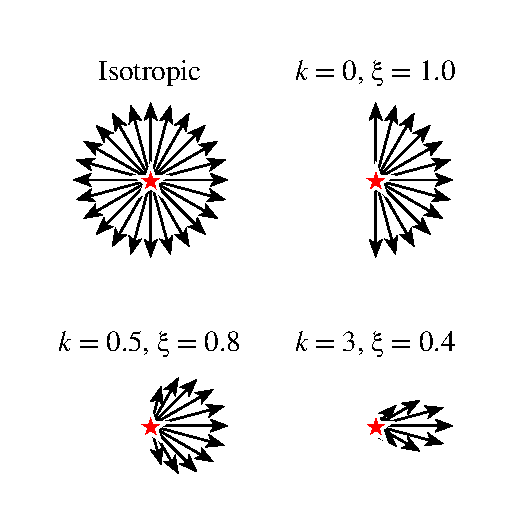
\includegraphics[width=0.5\linewidth]{./Figures/anisotropic-arrows}
  \label{fig:isotropic-aniso}
  \caption{Representaci\'on esquem\'atica de vientos con diferentes
    anisotrop\'ias:
    Arriba izquierda: Viento isotr\'opico esf\érico. Arriba derecha: viento
    isotr\'opico hemisf\'erico. Abajo: Vientos anisotr\'opicos donde el
    par\'ametro $k$ indica el grado de anisotrop\'ia (ver secci\'on
    \ref{sec:hipersonica})}
\end{figure}
\begin{figure}
  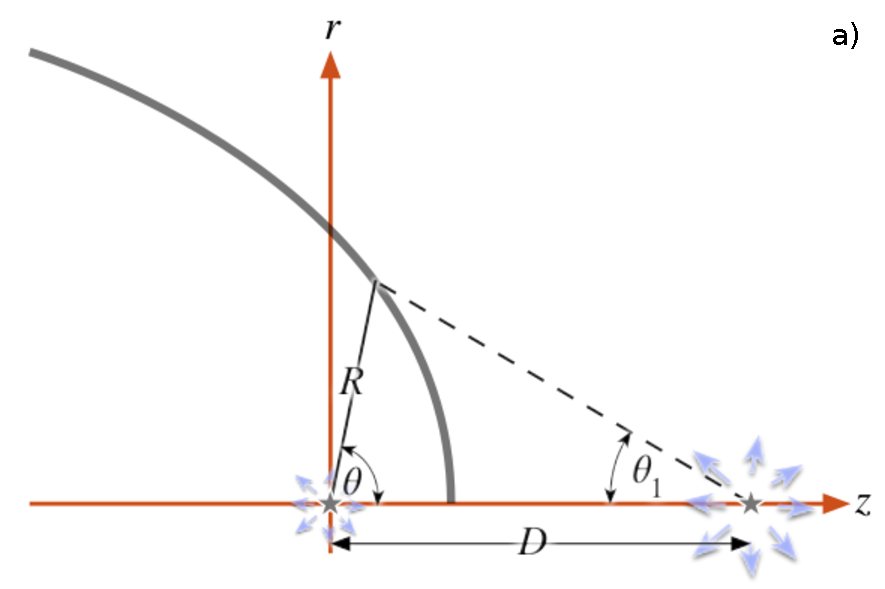
\includegraphics[width=0.5\linewidth]{./Figures/bowshock-crw-variables}
  \label{fig:crw-esquema}
\end{figure}

\subsection{Radios ``Caracter\'isticos''}

Las cantidades medibles que nos ayudan a caracterizar un choque de proa las
llamamos ``Radios caracter\'isticos'' (ilustrados en la figura
\ref{fig:char-radii}):
\begin{itemize}
\item Radio del choque en la direcci\'on del eje de simetr\'ia del sistema.
  Denotado como $R_0$
\item Radio en direcci\'on perpendicular al eje de simetr\'ia del sistema.
  Denotado como $R_{90}$
\item Radio de curvatura en la ``nariz'' del choque de proa. Denotado
  como$ R_c$
\end{itemize}

\begin{figure}
  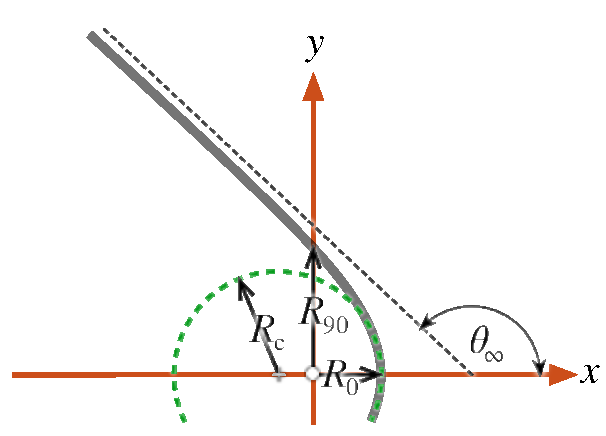
\includegraphics[width=\linewidth]{./Figures/characteristic-radii}
  \label{fig:char-radii}
  \caption{Representaci\'on esquem\'atica de los radios caracter\'isticos
  de un choque de proa}
\end{figure}



\section{Proyecci\'on en el Plano del Cielo}

Para un choque de proa que es la vez geom\'etricamente delgado y
\'opticamente delgado, \'unicamente se observa el borde de \'este por
abrillantamiento al limbo, por lo tanto, sua orientaci\'on respecto a
la l\'inea de visi\'on modifica su forma respecto a la forma real del
choque. Para ello, rotamos el sistema de referencia del choque de proa
en coordenadas cartesianas, denotado por $(x, y, z)$, por un \'angulo
que llamamos \textit{inclinaci\'on}, denotado por $i$, en el plano $xz$,
de modo que la transformaci\'on entre el sistema de refencia del choque
y el sistema de referencia del plano del cielo, denotado por
$(x', y', z')$ queda como sigue:

\begin{align}
  \left(
  \begin{array}{c}
    x' \\ y' \\ z'
  \end{array}
  \right) &=
  \left(
  \begin{array}{c}
    x\cos i - z\sin i \\ y' \\ z\cos i + x\sin i
  \end{array}
  \right)
  \label{eq:rotation}
\end{align}

Por otro lado, la forma tridimensional del choque de proa viene dado por:

\begin{align}
  \left(
  \begin{array}{c}
    x \\ y \\ z
  \end{array}
  \right) &=
            R(\theta)\left(
            \begin{array}{c}
              \cos\theta \\
              \sin\theta\cos\phi \\
              \sin\theta\sin\phi
            \end{array}
            \right)
\end{align}
La relaci\'on entre ambos sistemas de referencia se ilustra en la figura
\ref{fig:reference}.

\begin{figure}
  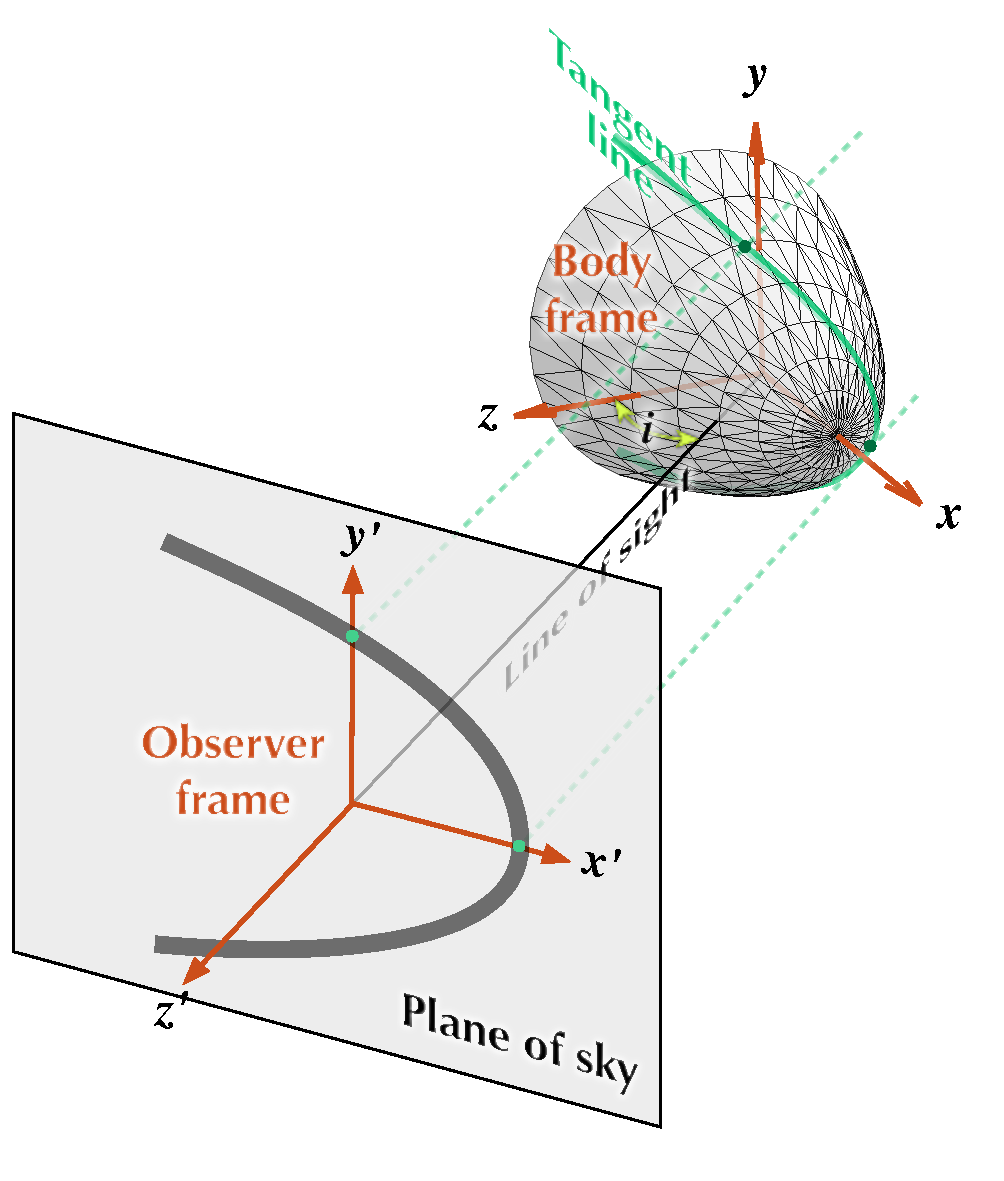
\includegraphics[width=\linewidth]{./Figures/projection-pos}
  \label{fig:reference}
  \caption{Sistema de referencia del choque vs sistema de referencia del
    plano del cielo. Los ejes $x'$ y $y'$ se encuentran en el plano del
    cielo, mientras el eje $z'$ es paralelo a la línea de visión.
    Solo la regi\'on del choque cuya tangente sea paralela a la l\'inea
    de visión será visible por abrillantamiento al limbo.}
\end{figure}

\subsection{Vectores normal y tangente a la superficie}

Si definimos los vectores $\hat{n}$ y $\hat{t}$, como los vectores
normal y tangente a la superficie, respectivamente para $\phi$ constante.
En el caso $\phi = 0$ (figura \ref{fig:unit-vec}), ambos vectores se encuentran
en el plano $xy$ y es fácil mostrar que:

\begin{align}
  \hat{t}_0 =
  \left(
  \begin{array}{c}
    -\cos\alpha \\
    \sin\alpha \\
    0
  \end{array}
  \right)
  \quad \mathrm{y} \quad
  \hat{n}_0 =
  \left(
  \begin{array}{c}
    \sin\alpha \\
    \cos\alpha \\
    0
  \end{array}
  \right)
  \label{eq:unit-vec}
\end{align}

Donde:
\begin{align}
  \tan\alpha = -\frac{dy}{dx} = \frac{1+\omega\tan\theta}{\tan\theta-\omega}
\end{align}
y:
\begin{align}
  \omega(\theta) = -\frac{1}{R}\frac{dR}{d\theta} 
\end{align}

Para otros valores de $\phi$, basta con hacer una rotación de las ecuaciones
(\ref{eq:unit-vec}) alrededor del eje $x$. Para la conversión al sistema de
referencia del plano del cielo se utiliza la ecuación (\ref{eq:rotation}):

\begin{align}
  \hat{n}' &= \frac{1}{\left(1 + \omega^2\right)^{1/2}} \\
           & \times \left(
             \begin{array}{c}
               (\cos\theta+\omega\sin\theta)\cos i-(\sin\theta-\omega\cos\theta)\sin i\sin\phi\\
               (\sin\theta-\omega\cos\theta)\cos\phi \\
               (\cos\theta+\omega\sin\theta)\sin i+(\sin\theta-\omega\cos\theta)\sin\phi\cos i
             \end{array}
                    \right) \\
    \hat{t}' &= \frac{1}{\left(1 + \omega^2\right)^{1/2}} \\
           & \times \left(
             \begin{array}{c}
               -(\sin\theta-\omega\cos\theta)\cos i-(\cos\theta+\omega\sin\theta)\sin i\sin\phi\\
               (\cos\theta+\omega\sin\theta)\cos\phi \\
               -(\cos\theta+\omega\sin\theta)\sin i+(\sin\theta-\omega\cos\theta)\sin\phi\cos i
             \end{array}
             \right) 
\end{align}


\begin{figure}
  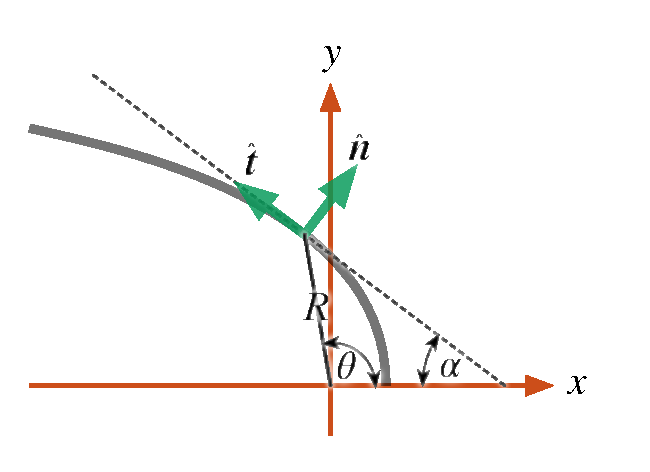
\includegraphics[width=0.8\linewidth]{./Figures/bowshock-unit-vectors}
  \label{fig:unit-vec}
  \caption{Vectores unitarios normal y tangente a la superficie $R(\theta)$
    en un plano de azimuth $\phi$ constante.}
\end{figure}


\subsection{Línea tangente}

Debido a que el choque es \'opticamente delgado y geom\'etricamente
delgado, solo la regi\'on del choque cuya tangente sea paralela a la
l\'inea de visi\'on ser\'a visible. Esto corresponde a una curva que
denominamos \textit{l\'inea tangente}, que debe cumplir con la siguiente
condición:

\begin{align}
  \hat{n}'\boldsymbol{\cdot} \hat{z}' = 0
\end{align}

Denotamos como $\phi_T$ al ángulo azimutal que cumple la condición anterior
para una inclinación dada, en función del ángulo polar $\theta$:
\begin{align}
  \sin\phi_T = \tan i\tan\alpha = \tan i\frac{1+\omega\tan\theta}{\omega-\tan\theta}
  \label{eq:phi-tan}
\end{align}
De esta manera, la forma de la línea tangente del choque de proa, a la que llamamos
\textit{forma proyectada} viene dada por:

\begin{align}
  \left(
  \begin{array}{c}
    x'_T \\
    y'_T \\
    z'_T
  \end{array}
  \right) =
  R(\theta)\left(
  \begin{array}{c}
    \cos\theta\cos i - \sin\theta\sin\phi_t\sin i \\
    \sin\theta\left(1-\sin^2\phi_T\right)^{1/2} \\
    \cos\theta\sin i + \sin\theta\sin\phi_T\cos i
  \end{array}
  \right) \label{eq:proj-shape}
\end{align}
En el caso general, $z'_T$ no es una función lineal de $x'_t$ y $y'_T$, por lo que
la línea tangente no se encuentra en un plano.

La forma aparente $(x'_t, y'_T)$  de la línea tangente también puede escribirse
en coordenadas polares $(R', \theta')$, donde:
\begin{align}
  R'(\theta) = \left(x'_t^2 + y'_T^2\right)^{1/2} & \mathrm{y} & \tan\theta' = \frac{y'_T}{x'_T}
  \label{eq:polar}
\end{align}
Es de notar a su vez que la ecuación (\ref{phi-tan}) no tiene solución para valores
arbitrarios de $\theta$ y de la inclinación, puesto que se requiere que
$\left|\sin\phi_T\right| < 1$. Por tanto, la línea tangente solo existe para valores
de $\theta$ tales que $\theta < \theta_0$ donde $\theta_0$ es el valor de $\theta$ en
el eje de simetría de la línea tangente proyectada $(\theta'(\theta_0)) = 0$ y que se
obtiene de la siguiente ecuación implícita:
\begin{align}
  \tan\theta_0 = \frac{|\tan i| + \omega(\theta_0)}{1 - \omega(\theta_0)|\tan i|}
\end{align}
Esto implica que si el choque de proa es suficientemente ``abierto''
$(\alpha > \alpha_{min})$, entonces para inclinaciones tales que
$|i| > 90^\circ - \alpha_{min}$ no existirá la línea tangente para ningún valor de $\theta$,
es decir, el choque de proa se encontrará sufientemente ``de cara'' como para que ya no
parezca un chouque de proa para el observador.

\subsection{Radios característicos en el plano del cielo}

En orden de comparar la forma $R(\theta)$ con observaciones, es útil definir los radios
característicos $R'_0$ y $R'_{90}$
\section{Cuádricas de Revolución}

Buscamos adjuntar el paper ``quadrics bowshock''
